% Adriano Bassignana nov 2017
% Program for creating a linear index useful for the construction of a compass on a conical support
% The program can be modified and adapted for the construction of other types of numeric indexes.
% The font used is OCR-B which allows to have alphabetic and numeric symbols very similar to those used in analogue flight gauges in the 50s and 80s
% You must have installed OCR-B in OTF format that has a GPL-2 and later compatible license.
% The font for Debian-Ubuntu systems can be downloaded as a ``texlive-fonts-extra'' package
% Ref: https://ctan.org/tex-archive/fonts/ocr-b/
\documentclass{standalone}
\usepackage{ocr}
\usepackage{tikz}
\tikzset{font={\fontsize{18pt}{10}\selectfont}}
\begin{document}
{\fontfamily{ocrb10f}\selectfont
    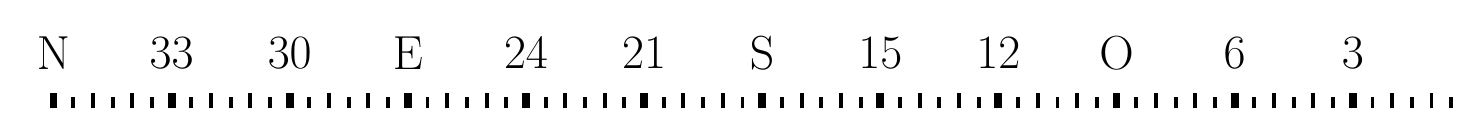
\begin{tikzpicture}[xscale=0.05]
      %5° Rays
      \foreach \a in {0, 5,...,355}
	\draw[line width=0.5mm] (\a,0) -- (\a,1.5mm);
      %10° Rays
      \foreach \a in {0, 10,...,350}
	\draw[line width=0.5mm] (\a,0) -- (\a,2.0mm);      
      %30° Rays
      \foreach \a in {0, 30,...,345}
	\draw[line width=1mm] (\a,0) -- (\a,2.0mm); 
      %labels  
      \draw (30,0.7) node {33};
      \draw (60,0.7) node {30};
      \draw (120,0.7) node {24};
      \draw (150,0.7) node {21};
      \draw (210,0.7) node {15};
      \draw (240,0.7) node {12};
      \draw (300,0.7) node {6};
      \draw (330,0.7) node {3};
      \draw (0,0.7) node {N};
      \draw (90,0.7) node {E};
      \draw (180,0.7) node {S};
      \draw (270,0.7) node {O};
    \end{tikzpicture}
}
\end{document}
